\chapter{Evaluation}
\label{chap:evaluation}
In this chapter, we evaluate our clustering implementation. We begin by defining the topologies and the metrics we use. We continue with an evaluation of our clustering parameters, where we determine what configurations of the parameters yield the most reliable and stable network, for different topologies. Next, we compare our clustering implementation to the \atwo{} system. We end this chapter with a discussion on the evaluation results, how our limitation on fault tolerance affected our results, and running different applications in a clustered network.


\section{Evaluation Setup}
We run several different tests to evaluate our clustering implementation. In this section, we describe our test setup, the network topologies we run our tests on, and the metrics we use. 

\subsection{The Cooja Simulator}
\label{subsec:cooja-setup}
Cooja \cite{Osterlind2006-cooja-introduction} is a simulator for ContikiOS \cite{Dunkels2004-contiki-introduction}, the operating system that Chaos and \atwo{} are implemented on \cite{chaos-introduction-paper, a2-introduction-paper}. In Cooja, we create networks with 50 and 200 nodes placed randomly in topologies of different sizes, to get both dense and sparse networks. We start with 50 nodes in a 100x100 $m^2$ area and increase the side of the square in steps of 300 meters up to 2500x2500 $m^2$. We do the same for 200 nodes but only up to 1300x1300 $m^2$. We only have one network topology per area and number of nodes. We simulate each test for 30 minutes, which gives us 600 rounds of data. 

We run most of our tests using 50 nodes for two reasons. First, 50 nodes are enough to see that the Clustering service creates several clusters. Second, running these simulations takes a significant amount of time, and it does not scale well when increasing the number of nodes. Simulating 30 minutes with 50 nodes takes 2-3 hours, and 200 nodes takes 30-50 hours on our hardware. However, when comparing our clustering process to the \atwo{} system, we also simulate 200 nodes to see the effects of scaling up the network. Moreover, we chose the different sizes from the fact that in Cooja, a network with an area of 100x100 $m^2$ ensures that is is a 1-hop network and at 2500x2500 $m^2$ the network is at least a 7-hop network.

\subsection{The Flocklab Testbed}
The Flocklab testbed \cite{Lim2013-flocklab-introduction} consists of 27 nodes deployed both indoors and outdoors at ETH Zurich. Flocklab provides several services that make it easy to measure and evaluate the code that is running on the nodes. Our tests log data to the serial port of an observer node, Flocklab aggregates the data and sends it to us at the end of each test. 


\subsection{Metrics}
\begin{newtext}
To define the metrics we use, we make a distinction between rounds which execute coordination and rounds which execute applications. Coordination is rounds in which the network is set up to enable applications to run; coordination includes the Cluster, Join, and Demote services. We also differentiate between static and dynamic coordination. Static coordination is scheduled at fixed round intervals to, for example, cluster the network. Dynamic coordination, on the other hand, is scheduled by nodes as needed during the application phase, to handle faults in the network or new nodes. Applications are programs that run with the goal of providing some value or perform some calculation; Some examples of applications are finding the maximum or mean of all values proposed by nodes in the network, or performing a two-phase commit.

We consider four metrics when evaluating clustering on \atwo{}: stability, reliability, latency, and energy usage. We define the metrics for one execution of a network, that is, one simulation in Cooja or one run on the Flocklab testbed.


\paragraph*{Stability} is a measurement of how often topology changes occur. We say that a node is stable if it is executing an application and unstable if it is executing dynamic coordination. Stability during one round is the proportion of nodes that are stable. We give the following definition for the stability for one test. 


\begin{Definitions}{}{}
Let $s_i$ be the set of stable nodes in round $i$, $n$ the set of all nodes, and $R$ the set of all rounds which do not execute static coordination.

\begin{equation*}
    Stability = \frac{\sum\limits_{i \in R}{|s_i|}}{|n|*|R|}
\end{equation*}

\end{Definitions}

\paragraph*{Reliability} is a measurement of how well an application runs on the network; thus, it is only measured during application rounds. Reliability during one round is the proportion of stable nodes that successfully execute an application. We give the following definition for the reliability for one test.

\begin{Definitions}{}{}
Let $a_i$, $a_i \subset s_i$, be the set of stable nodes that succeeds with an application in round $i$, and $R_a$ the set of all rounds in which an application is executed.


\begin{equation*}
    Reliability = \frac{\sum\limits_{i \in R_a}{|a_i|}}{\sum\limits_{i \in R_a}{|s_i|}}
\end{equation*}

\end{Definitions}


\paragraph*{Latency} is a measurement of how long it takes for an application to terminate. For a stable node in one round, latency is the number of slots from the start of the round until the node powers down. We give the following definition for the latency for one test.

\begin{Definitions}{}{}
Let $l_{ij}$ be the latency for node $j$ in round $i$.

\begin{equation*}
    Latency = \frac{\sum\limits_{i \in R_a}{ \sum\limits_{j \in s_i}{l_{ij} } }}{\sum\limits_{i \in R_a}|s_i|}
\end{equation*}
\end{Definitions}


\paragraph*{Energy usage} is a measurement of the average amount of energy used by a node per Energest time unit. Energest is the built-in energy estimation module in Contiki and we measure energy usage in all rounds, both during coordination and applications. We give the following definition for the energy usage for one test.


\begin{Definitions}{}{}
Let $e_{i}$ be the energy used by node $i$ in one test, and let $T$ be the running time of the test in Energest time units.

\begin{equation*}
    Energy\ usage = \frac{\sum\limits_{i \in n}{e_{i}}}{T*n}
\end{equation*}
\end{Definitions}

\end{newtext}

\subsection{Limitations}
We impose several limitations on the evaluation of our clustering implementation. We only run tests in the Cooja simulator and on the Flocklab testbed. Running simulations gives us the freedom to choose topologies, but the simulations do not model the network perfectly. Flocklab, on the other hand, contains real nodes but is relatively small with only 27 nodes in a static configuration. We only compare our implementation to \atwo{}, and do not consider any other WSN protocols.

Furthermore, we only simulate two different network sizes, 50 nodes and 200 nodes. We only simulate 50 nodes when searching for parameter values, and include networks with 200 nodes when we compare our clustering process to \atwo{}.

To limit the scope of our parameter evaluation, we use the values listed in \cref{tab:parameter-default-values} for the parameters that we are not currently evaluating.

\begin{table}[bt]
\centering
\caption{The parameters we evaluate and their default values}
\label{tab:parameter-default-values}
\begin{tabular}{r|l}
\textbf{Parameter}                 & \textbf{Value} \\ \hline
Competition Radius                 & 1              \\
Minimum cluster size                 & 4              \\
Nodes per cluster ratio            & 10             \\
Round re-synchronisation threshold & 3             
\end{tabular}
\end{table}

Lastly, we only evaluate clustering using the Max application. The Max application is the most straightforward application currently implemented in the \atwo{} system. We discuss how to apply different applications and the implications of doing so in \cref{subsec:discuss-other-apps}.


\section{Clustering Parameters}
\label{sec:clustering-parameters}
In this section, we experimentally search for optimal values to the parameters in our clustering algorithm. The parameters are \emph{round re-synchronisation threshold}, \emph{competition radius}, \emph{minimum cluster size}, and \emph{nodes per cluster ratio}. We run each parameter configuration three or six times and plot the reliability and stability of each test for each network topology.

We only look at the reliability and stability of these tests since the purpose is to find which parameters yield the best results, in terms of running the application. However, we include the latency results in \cref{app:a} for completeness; we note that there are no significant differences in latency for different values of these parameters, and will not comment on these results any further.

We use a different number of topologies depending on which parameter we evaluate. When evaluating competition radius, we test on all network topologies we describe in \cref{subsec:cooja-setup} since this parameter is dependent on the density of the network. However, when we test the parameters minimum cluster size and nodes per cluster ratio, we use topologies from 100x100 $m^2$ to 1300x1300 $m^2$, using competition radius 1. We argue that increasing the competition radius while simultaneously increasing the area of the networks will not give any new results. By excluding the network topologies with a larger area, we could repeat each configuration for these tests a total of six times, instead of three.

\subsection{Round Re-synchronisation Threshold}
\label{subsec-resync-threshold}
The \emph{round re-sync threshold} parameter is not directly related to the clustering process. Rather, it is a setting that controls a fundamental part of the \atwo{} system. Round re-sync threshold is a numeric parameter that determines how many rounds a node will spend receiving no packets before associating with the network again. 

We evaluate three different values of the round re-sync threshold (1, 2, and 3), for each value of re-sync threshold we evaluate three different values of competition radius (1, 2, and 3), which gives us a total of 9 test configurations. We use different values of competition radius for these tests because we do not want a suboptimal competition radius to affect the results regarding the re-sync threshold, especially for sparser networks.

\begin{newtext}
We make two observations from the round re-sync threshold results, shown in \cref{fig:resync-treshold-tests}. First, the reliability is drastically increased when the re-sync threshold is greater than 1. Second, the stability increases as the re-sync threshold increases. 

The reason reliability is low when the re-sync threshold is 1 (\cref{subfig:resync-treshold-1}), is that a clustered network is not compatible with such a low threshold. The cause of this problem is that the network has a single initiator during CH rounds, which is the CH with the lowest ID. Furthermore, we allow clusters to schedule and run the Join service during CH rounds, meaning those clusters will not participate with their value, neither will they forward packets during CH rounds. 

The problem, which often occurs, is that the cluster with the lowest ID runs the Join service during a CH round, in that case, there is no initiator present for the CH round. Without an initiator, all other clusters that participate in the CH round, will increase their resynchronisation counter by one, reach the resynchronisation threshold, and start associating. Furthermore, as we discuss in \cref{section:evaluation-discussion}, our limitation regarding fault tolerance further exacerbates this problem.

Usually, these scenarios only affect the stability of the network. However, in this case, the reliability is also affected since the network never has a chance to continue normal execution. Since the re-sync threshold is set too low, there is a high probability that every round has some portion of nodes associating, and some portion of nodes running the max application but failing since the only initiator is running the Join service.

\end{newtext}

\begin{newtext}
Furthermore, the stability increases with the re-sync threshold. The increase in stability when increasing the parameter from 1 to 2 follows from the same reasoning as for the reliability. However, the stability continues to increase when going from 2 to 3 as well. With an increase in the re-sync threshold, there is a lower chance that a node will associate with the network since it has a higher chance of receiving at least one valid packet before it reaches the threshold. Thus we see an increase in stability since in a network with a higher re-sync threshold nodes will wait longer before recognising a bad connection and try to re-associate.
\end{newtext}

From this evaluation, we conclude that out of the values we tested, using a re-sync threshold of 3 gives the best results. Even though \cref{fig:resync-treshold-tests} imply a trend of higher stability with an increasing re-sync threshold. However, we did not test greater values of this parameter due to time constraints, we discuss implications of increasing it more in \cref{discussion:clustering-parameters}. All further evaluation of our clustering implementation uses a re-synchronisation threshold of 3.

\begin{figure}[H]
\centering
\begin{subfigure}{\textwidth}
    \centering
    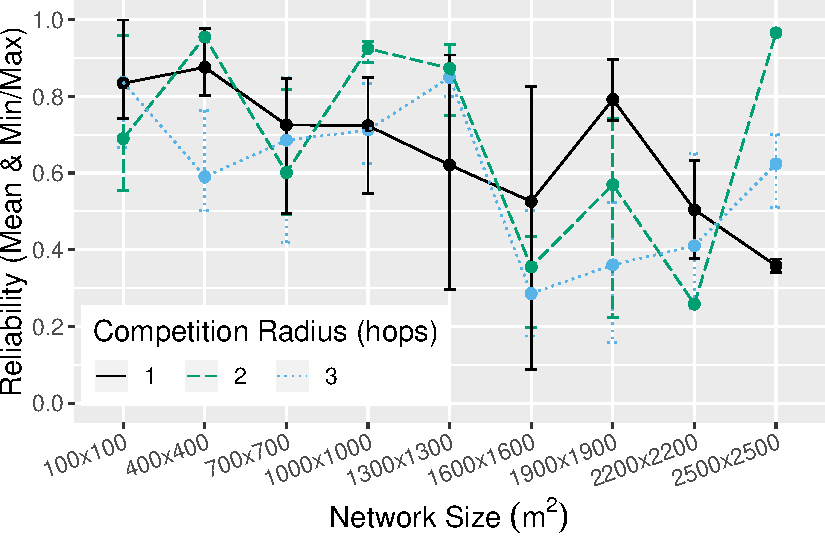
\includegraphics[width=0.49\textwidth, keepaspectratio]{figure/Results/ParameterEvaluation/ResyncThreshold1_Reliability.pdf}
    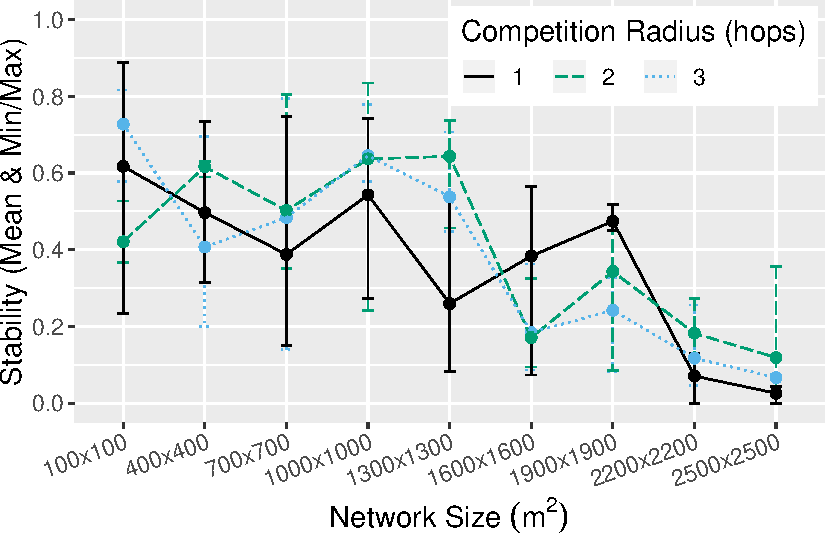
\includegraphics[width=0.49\textwidth, keepaspectratio]{figure/Results/ParameterEvaluation/ResyncThreshold1_Stability.pdf}
    \caption{Re-synchronisation threshold 1.}
    \label{subfig:resync-treshold-1}
\end{subfigure}
\begin{subfigure}{\textwidth}
    \centering
    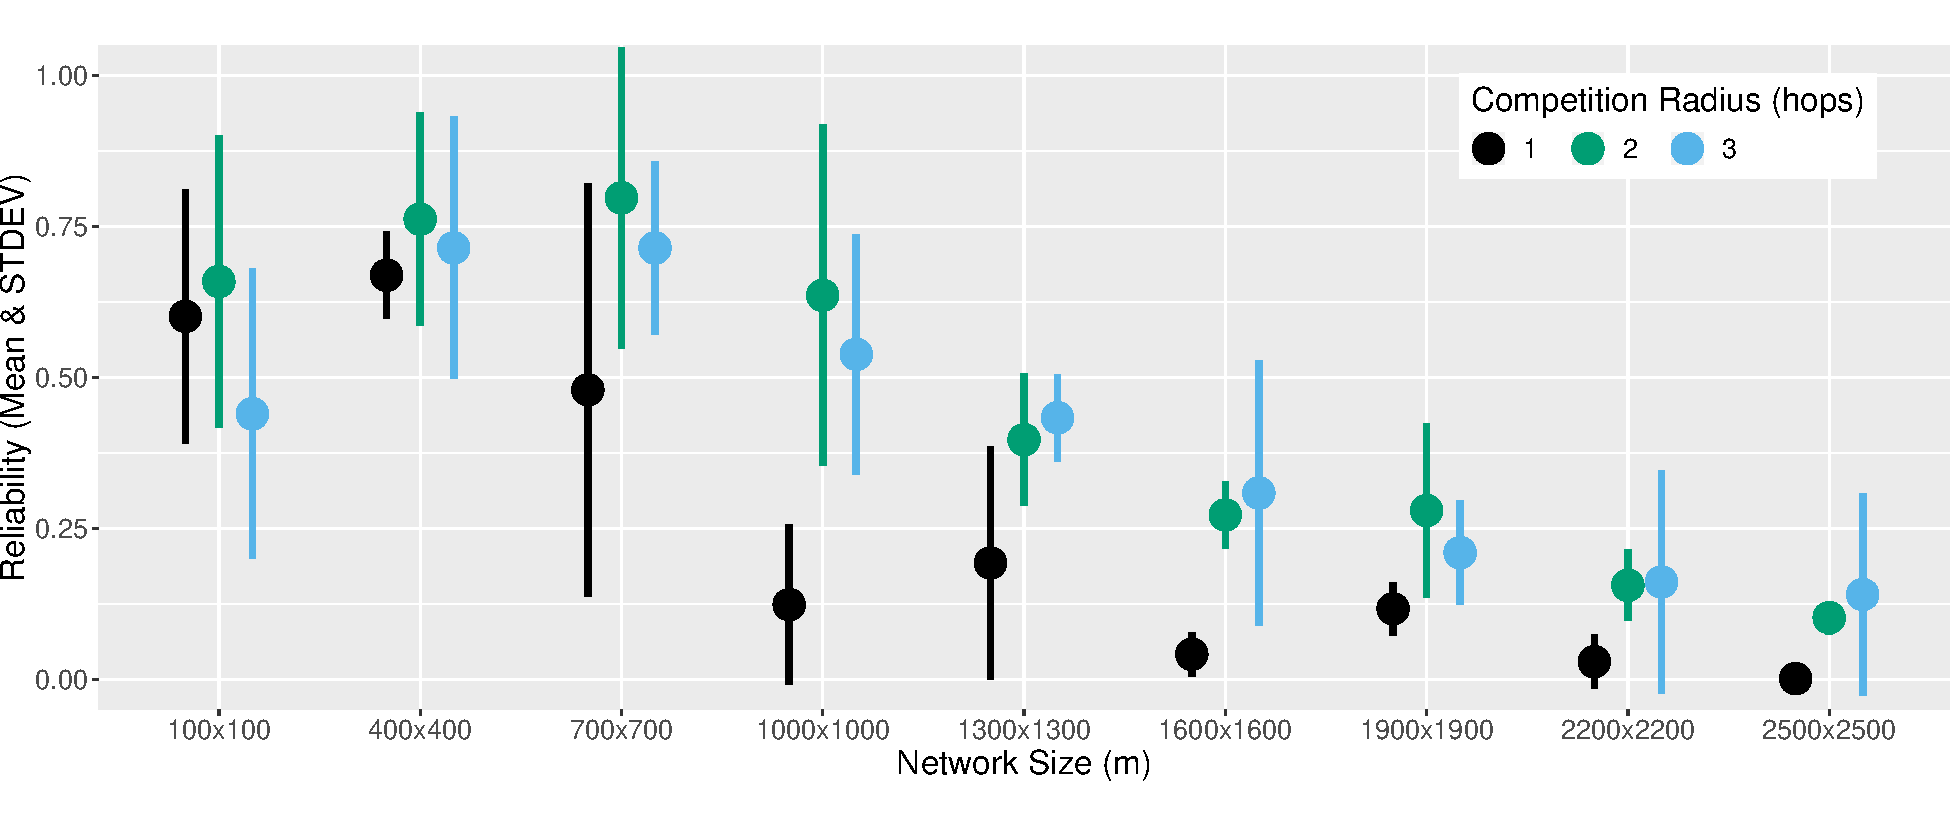
\includegraphics[width=0.49\textwidth, keepaspectratio]{figure/Results/ParameterEvaluation/ResyncThreshold2_Reliability.pdf}
    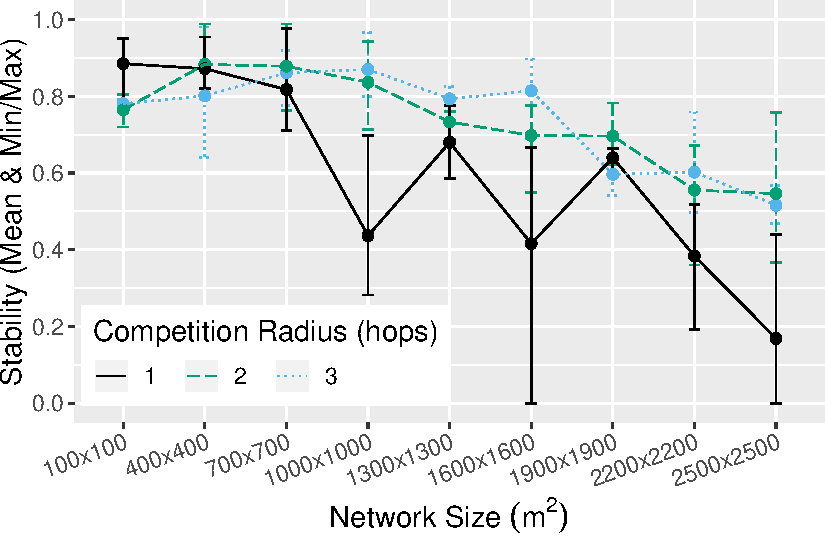
\includegraphics[width=0.49\textwidth, keepaspectratio]{figure/Results/ParameterEvaluation/ResyncThreshold2_Stability.pdf}
    \caption{Re-synchronisation threshold 2.}
    \label{subfig:resync-treshold-2}
\end{subfigure}
\begin{subfigure}{\textwidth}
    \centering
    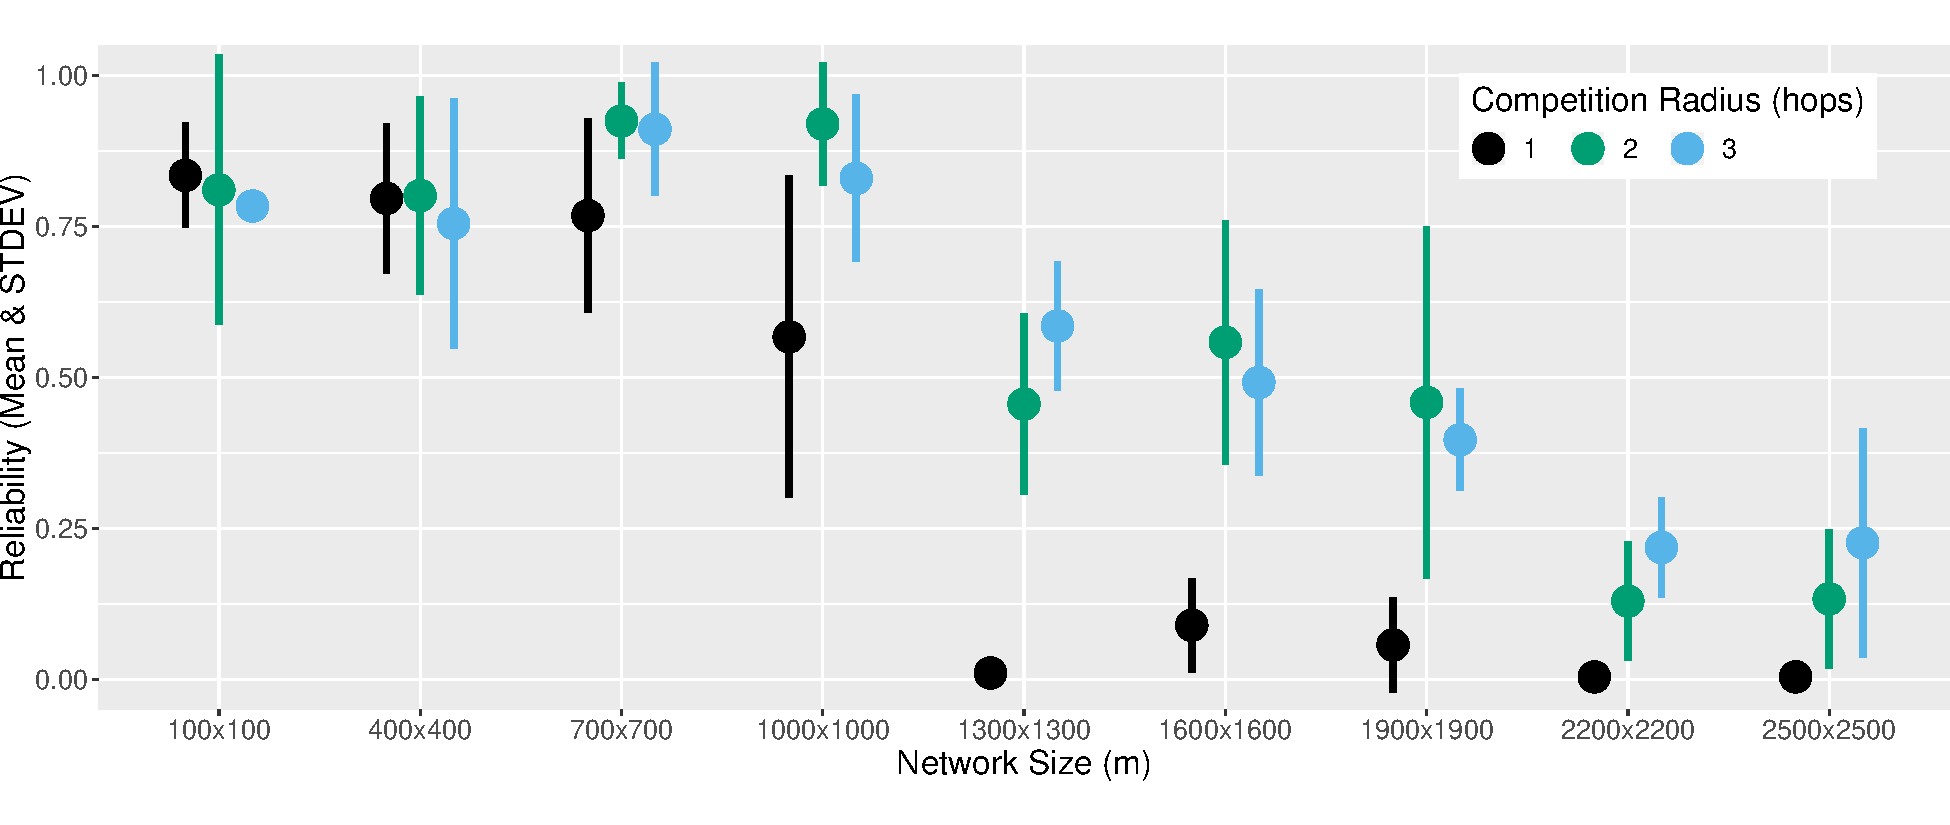
\includegraphics[width=0.49\textwidth, keepaspectratio]{figure/Results/ParameterEvaluation/ResyncThreshold3_Reliability.pdf}
    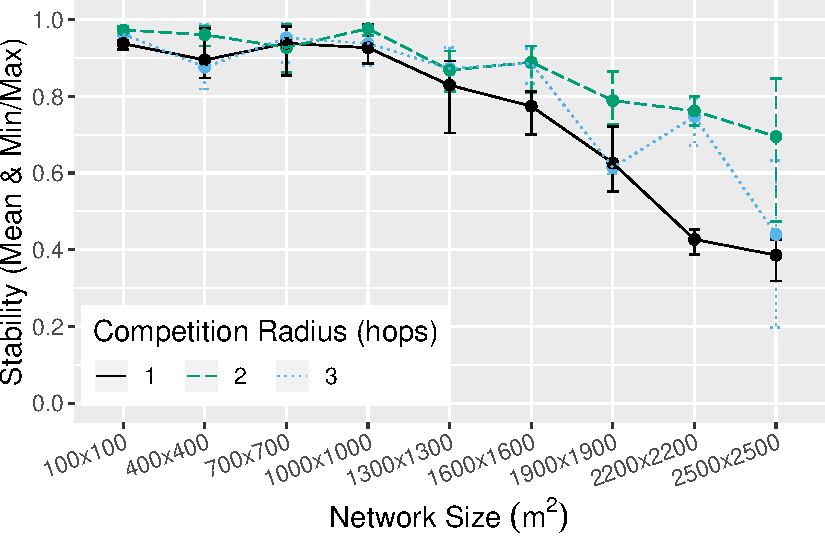
\includegraphics[width=0.49\textwidth, keepaspectratio]{figure/Results/ParameterEvaluation/ResyncThreshold3_Stability.pdf}
    \caption{Re-synchronisation threshold 3.}
    \label{subfig:resync-treshold-3}
\end{subfigure}

    \caption{Resynchronisation threshold tests for different values of Competition radius. Both reliability and stability increases as the re-sync threshold increases.}
    \label{fig:resync-treshold-tests}
\end{figure}


\begin{figure}[bt]
    \centering
    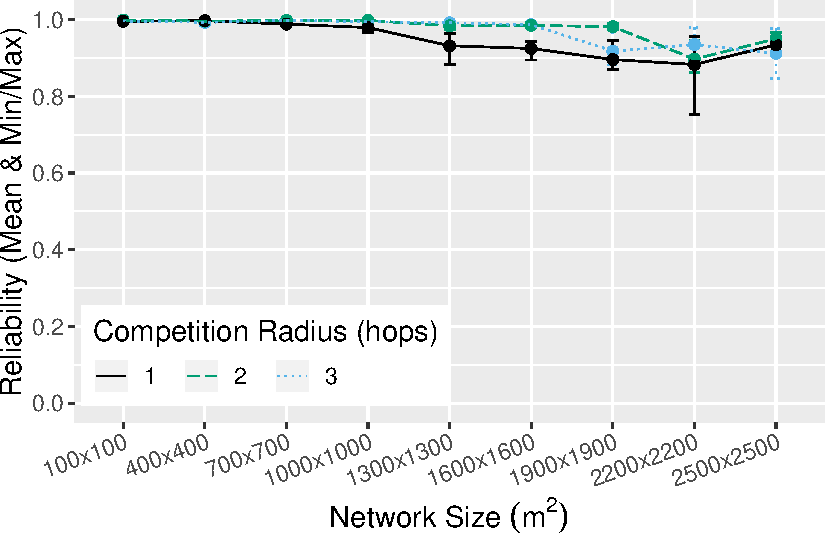
\includegraphics[width=0.49\textwidth, keepaspectratio]{figure/Results/ParameterEvaluation/CompetitionRadius_Reliability.pdf}
    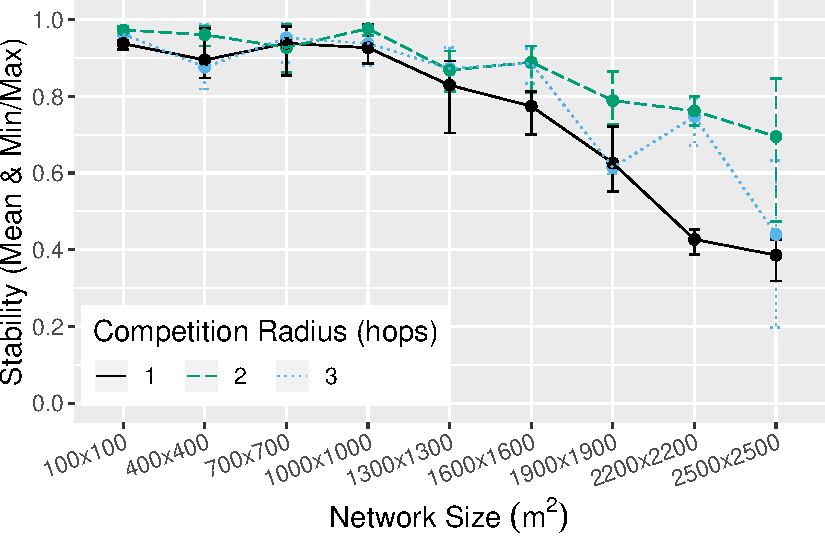
\includegraphics[width=0.49\textwidth, keepaspectratio]{figure/Results/ParameterEvaluation/CompetitionRadius_Stability.pdf}
    \caption{The reliability and stability for different network sizes. Each network size has been tested with competition radius 1, 2, and 3.}
    \label{fig:comp-radius-reliability}
\end{figure}

\subsection{Competition Radius}
\label{subsec:competition-radius}


\begin{newtext}
Competition radius determines the distance, in hops, from which a node can choose a CH. For this parameter, we evaluate the values 1, 2 and 3, which ensures that we test the minimum value of 1 but also not get too sparse clusters. We show the average, minimum, and maximum reliability and stability for each network size and each competition radius in \cref{fig:comp-radius-reliability}. Note that this figure is the same as \cref{subfig:resync-treshold-3} because we set the re-synchronisation threshold to 3 for all tests. Consequently, both of these tests use the same parameter values, so we did not rerun the test.

We see that both reliability and stability decreases as the size of the networks increase. We expect to see this decrease since clustering sparse networks will make them even sparser, which hinders communication. However, we see that higher values of competition radius are better for these networks since larger clusters are created, which does not impact communication as much as small clusters. Furthermore, the differences in stability and reliability for the denser networks (100x100, 400x400, and 700x700) is noise. These networks are 1-hop networks, and thus the competition radius value does not affect the clustering.
\end{newtext}

 
\subsection{Minimum Cluster Size}
Minimum cluster size determines the smallest cluster that is allowed to exist after the clustering process has converged on a set of clusters. All clusters with fewer nodes are removed, and the affected nodes join other clusters. We evaluate this parameter using three different values, 2, 4, and off; off means that no clusters are considered too small. We did not test any larger values for this parameter since we only use 50 nodes for the parameter tests, and a value larger than 4 would mean that more than 10\% of the nodes in the network could be in a cluster and it would be removed, which we consider too aggressive. We show the reliability and stability for these tests in \cref{fig:min-node-count-reliability}.

\begin{newtext}
When we look at the reliability for this parameter, we see that there is no significant difference for any topology or parameter value. However, we see a small variance in stability for larger networks. Looking at the data on how many cluster heads were created and demoted for these tests, which we can see in \cref{fig:minnodecount-chsafterdemotion}, we see two interesting results. First, using higher values of this parameter show no significant difference in the number of CHs created by the clustering process. Second, there was one test which demoted many more CHs than the others, the value 2 for the 100x100 $m^2$ topology. The high number of demoted CHs resulted in the CH count being close to the average. In that test, 32 CHs were demoted while normally 1-2 CHs are demoted. This recovery demonstrates that using this parameter can help the clustering process handle faults in the Clustering service. 
\end{newtext}



\begin{figure}[bt]
    \centering
    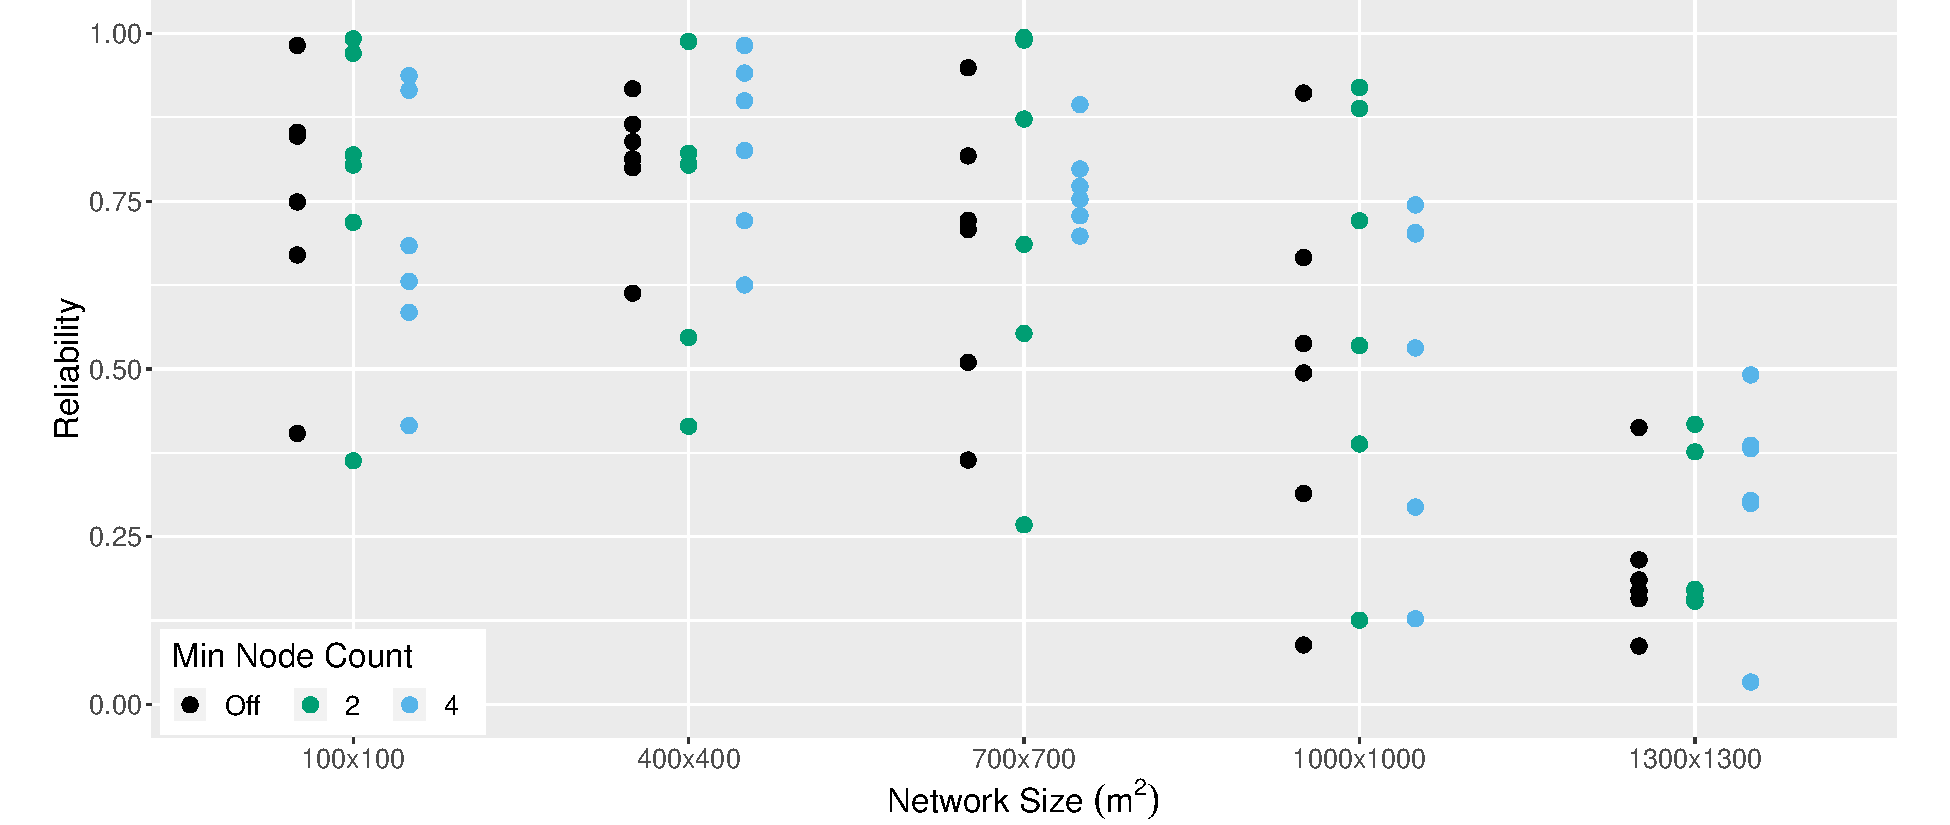
\includegraphics[width=0.49\textwidth, keepaspectratio]{figure/Results/ParameterEvaluation/MinNodeCount_Reliability.pdf}
    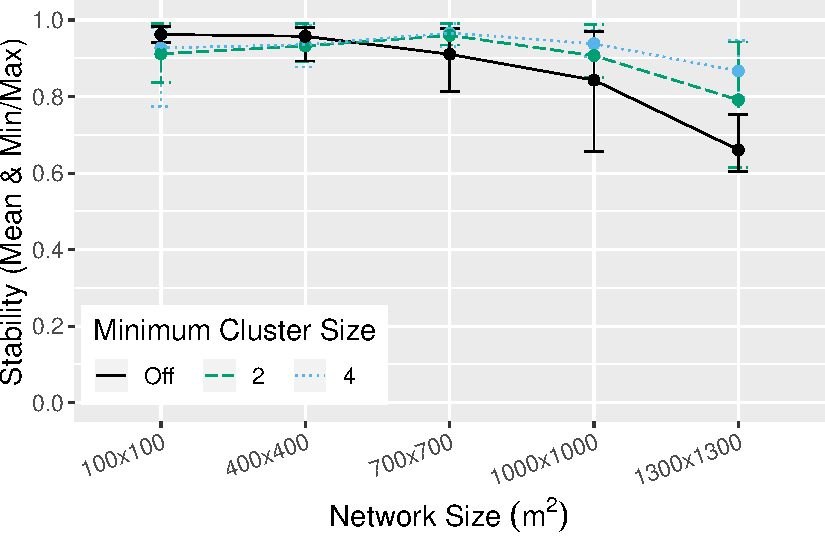
\includegraphics[width=0.49\textwidth, keepaspectratio]{figure/Results/ParameterEvaluation/MinNodeCount_Stability.pdf}
    \caption{The reliability and stability for different network sizes. Each network has been tested with minimum cluster size values off, 2, and 4.}
    \label{fig:min-node-count-reliability}
\end{figure}

\begin{figure}[bt]
    \centering
    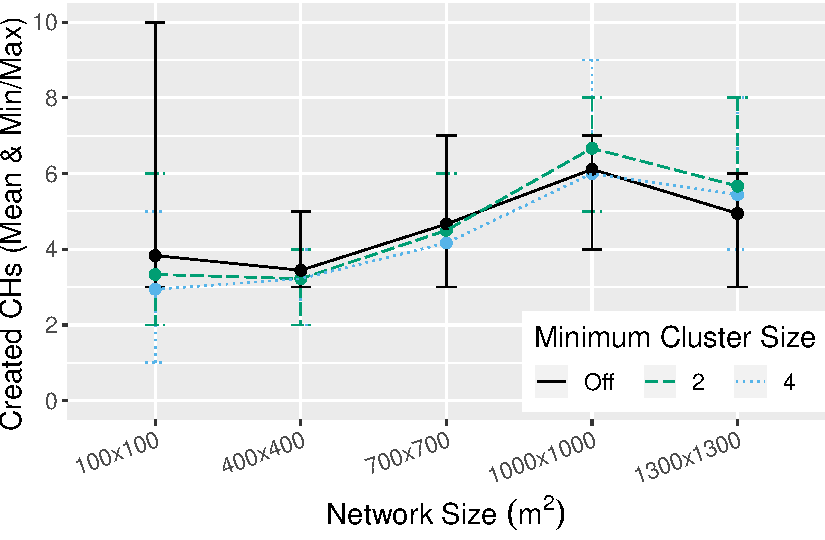
\includegraphics[width=0.49\textwidth, keepaspectratio]{figure/Results/ParameterEvaluation/MinNodeCount_CHsAfterDemotion.pdf}
    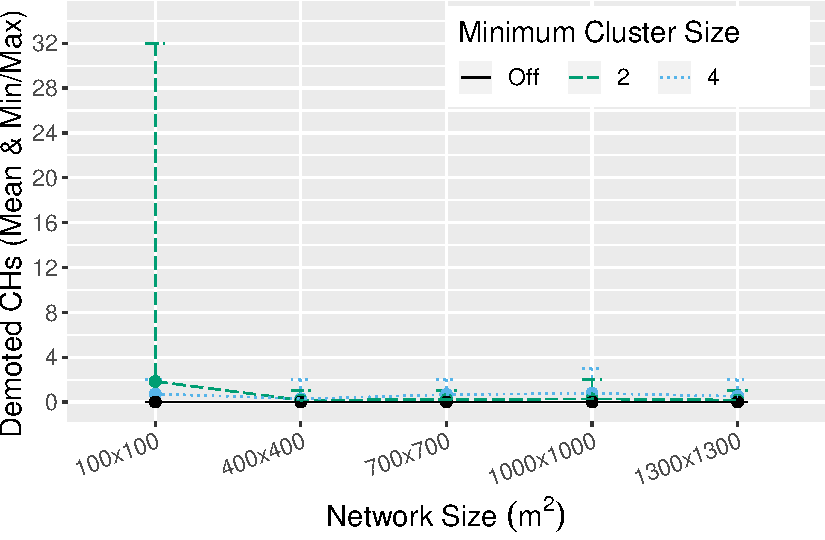
\includegraphics[width=0.49\textwidth, keepaspectratio]{figure/Results/ParameterEvaluation/MinNodeCount_DemotedCHs.pdf}
    \caption{Shows the number of CHs after the clustering process has finished, and the number of demoted CHs.}
    \label{fig:minnodecount-chsafterdemotion}
\end{figure}

\subsection{Nodes per Cluster Ratio}
\label{subsec:nodes-per-cluster-ratio}
The \emph{nodes per cluster ratio} parameter determines if nodes may become CHs even if they have heard from another CH within the competition radius. The parameter describes a ratio of how many neighbours a node needs to have relative to the number of CHs the node has heard. We test the values 5, 10, 15, and off for this parameter. The value off means a CH will never announce itself if it has heard from another CH within the network's competition radius. The results can be seen in \cref{fig:nodes-per-cluster-ratio-reliability}.

\begin{newtext}
The most significant results for the nodes per cluster ratio parameter is the decrease in stability and reliability in the 1000x1000 and 1300x1300 $m^2$ networks. With more clusters in networks with a larger area, we see more clusters failing with communication, causing nodes to try and re-synchronise, which is worsened by our limitation on fault tolerance. Furthermore, the two deviations in stability for 100x100 $m^2$ in the case of 10 and 15 nodes per cluster ratio are both due to noise.

Additionally, we see a small but constant decrease in reliability for the parameter value 5. This decrease is because the Clustering service creates too many clusters which are only demoted or otherwise removed, as can be seen in \cref{fig:nodes-per-cluster-ratio-promoted-ch-count}. Since demoting a CH may cause a fault, increasing the number of demotions will increase the probability of a fault to occur. Usually, these scenarios only affect the stability of the network, but in this case, the reliability is also affected since the CHs could not agree on which CHs was demoted and thus never agree on the correct maximum value in the CH rounds.

Nonetheless, we noticed that more nodes announced themselves as CH with a smaller nodes per cluster ratio value as seen in \cref{fig:nodes-per-cluster-ratio-promoted-ch-count}; this shows that the parameter works as intended but requires careful consideration when configured, and needs to be adapted to the network topology.

\end{newtext}

\begin{figure}[bt]
    \centering
    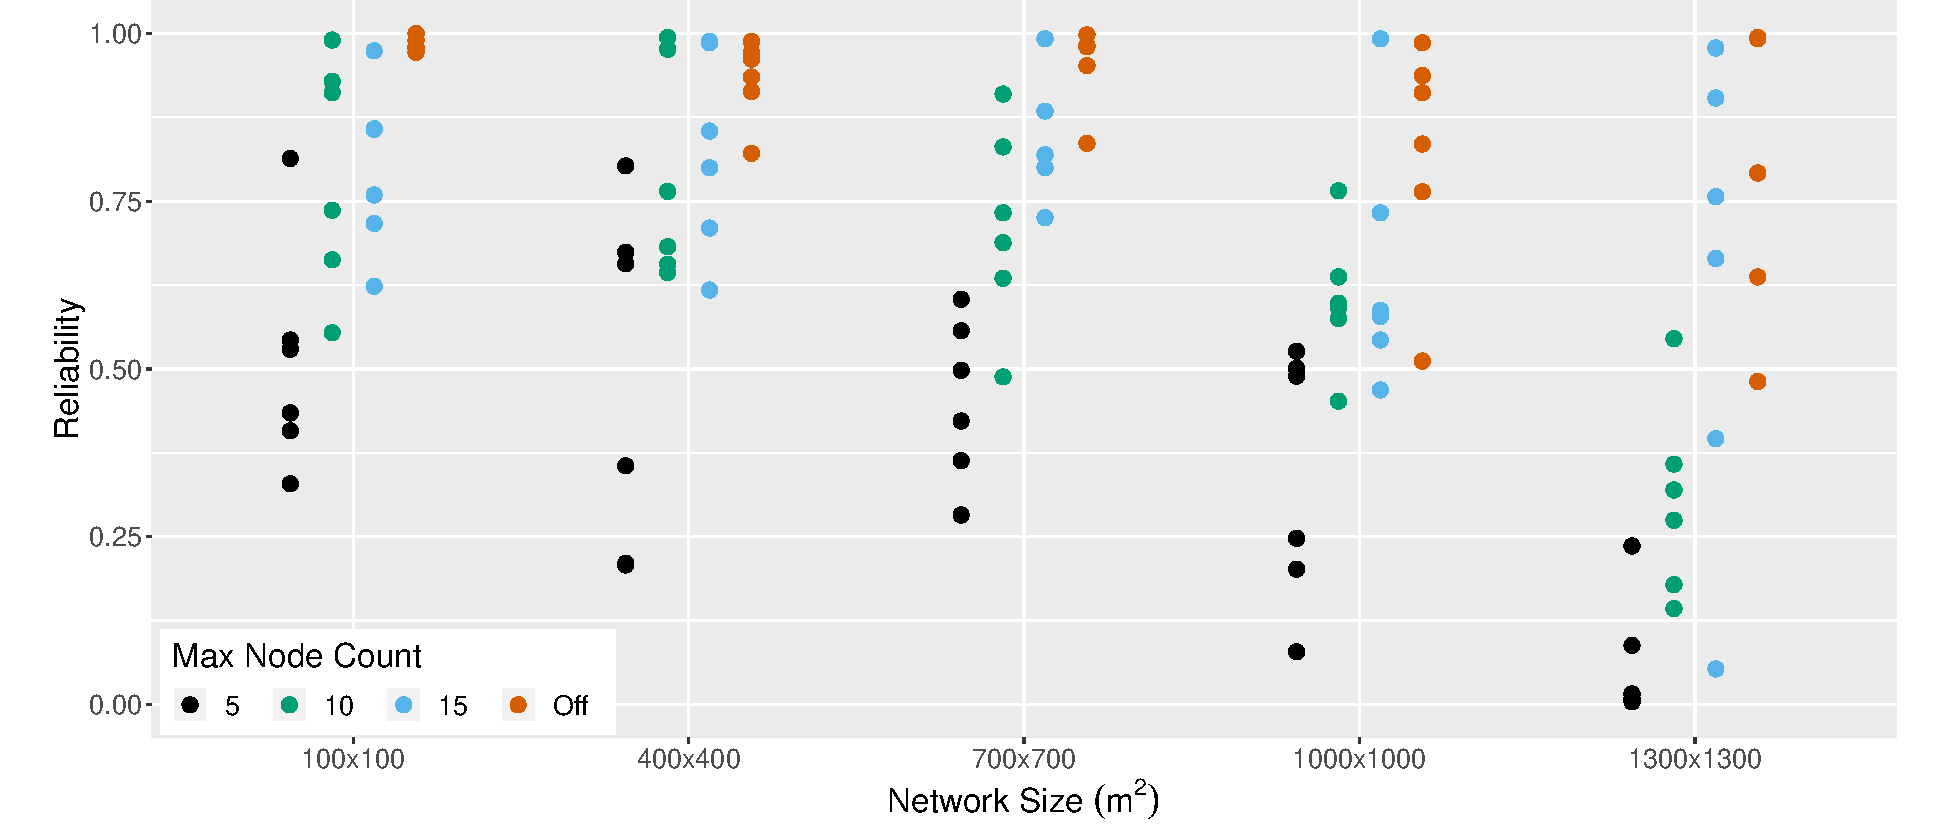
\includegraphics[width=0.49\textwidth, keepaspectratio]{figure/Results/ParameterEvaluation/MaxNodeCount_Reliability.pdf}
    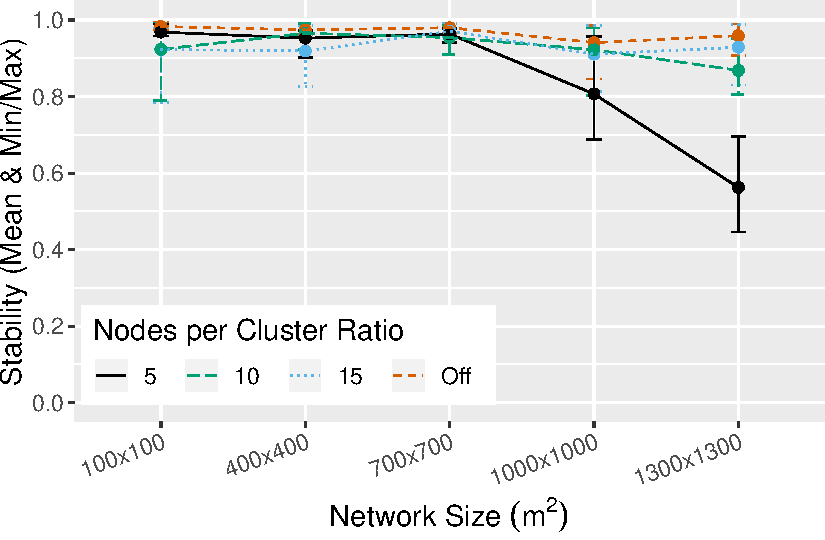
\includegraphics[width=0.49\textwidth, keepaspectratio]{figure/Results/ParameterEvaluation/MaxNodeCount_Stability.pdf}
    \caption{The reliability and stability for different network sizes. Each network size has been tested with max node count off, 5, 10, and 15.}
    \label{fig:nodes-per-cluster-ratio-reliability}

    \centering
    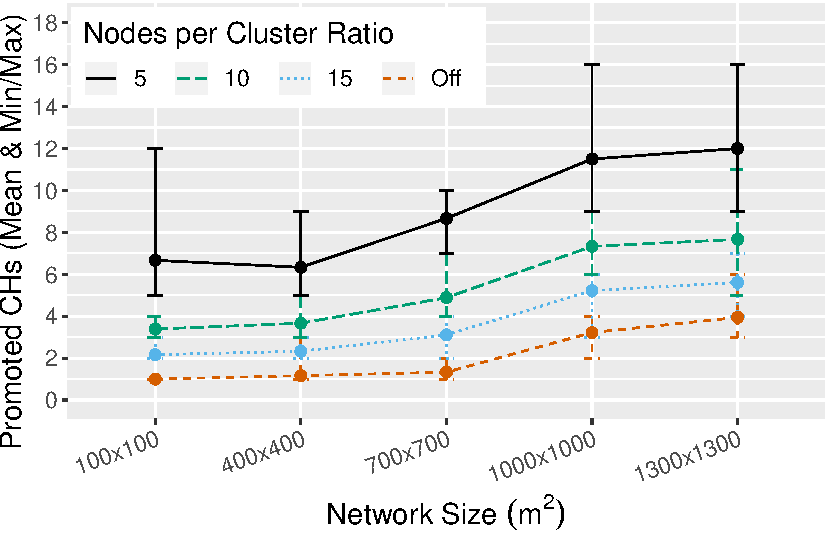
\includegraphics[width=0.49\textwidth, keepaspectratio]{figure/Results/ParameterEvaluation/MaxNodeCount_PromotedCHCount.pdf}
    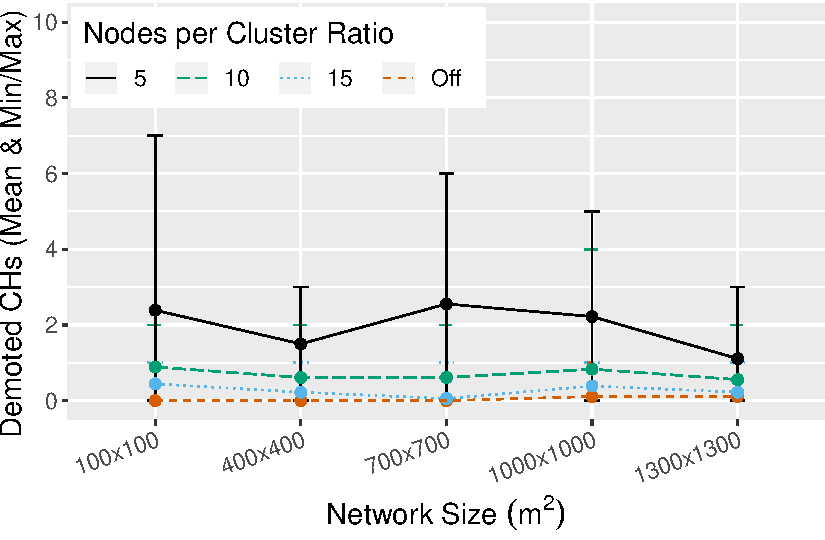
\includegraphics[width=0.49\textwidth, keepaspectratio]{figure/Results/ParameterEvaluation/MaxNodeCount_DemotedCHCount.pdf}
    \caption{The number of elected CHs before the Demote service runs, and the number of demoted CHs.}
    \label{fig:nodes-per-cluster-ratio-promoted-ch-count}
\end{figure}

\section{Comparing \atwo{} with Clustering}
\label{sec:comparing-a2-and-clustering}
In this section, we show the results of evaluating our clustering implementation and compare with the results from our evaluation of the original \atwo{} system. We show results for stability, reliability, latency, and estimated energy usage for all tests we run. We use different parameter values for some network topologies during this comparison. The most significant change is that we increase the competition radius as the network sizes increases. We list all parameter values for these tests in \cref{app:parameter-values-for-the-atwo-comparison}.


\subsection{Reliability and Stability}
\label{subsec:evaluation-reliability}
\begin{newtext}
We show reliability and stability for the evaluations with 50 nodes in \cref{subfig:reliability-50-nodes} and for 200 nodes in \cref{subfig:reliabilty-200-nodes}. Looking at the reliability for both of these, we see almost no difference for most network topologies, except with 50 nodes for 2200x2200 and 2500x2500 $m^2$, where the reliability drops when using clustering. The reason it drops is presented in detail \cref{subsec:competition-radius}, but essentially, too small clusters are created for these sparse networks.

However, the stability results have a higher variance. In the networks with 50 nodes, the clustered networks have lower stability, there are some tests which achieve similar levels of stability, but on average it is lower or much lower. In networks with 200 nodes, on the other hand, clustering achieves better results, the average stability is still lower than for the \atwo{} system, but there are some tests where clustering outperforms \atwo{} slightly. 

The reason \atwo{} drops in stability for 200 nodes, is that when one node loses connection with the network, the whole network has to spend on average, two or three rounds running the Join service. The clustering implementation, on the other hand, should only have to run the Join service locally in the affected cluster, which impacts stability less. However, since the clustering implementation lacks fault tolerance (discussed in \cref{section:evaluation-discussion}), the stability results for clustering are worse than they could be.

Furthermore, the stability has a decreasing trend in the 50 node networks while it is increasing in the 200 node networks. The reason the stability has an increasing trend in 200 node networks is that the small networks are dense and therefore generate more interference, which increases the number of faults that occur. However, we have not tested larger networks than 1300x1300 $m^2$ using 200 nodes, and it is possible that the stability will show a similar trend as the 50 nodes network when the area of the networks is increased further.

\end{newtext}
\begin{figure}[bt]
    \centering
    \begin{subfigure}{\textwidth}
            \centering
            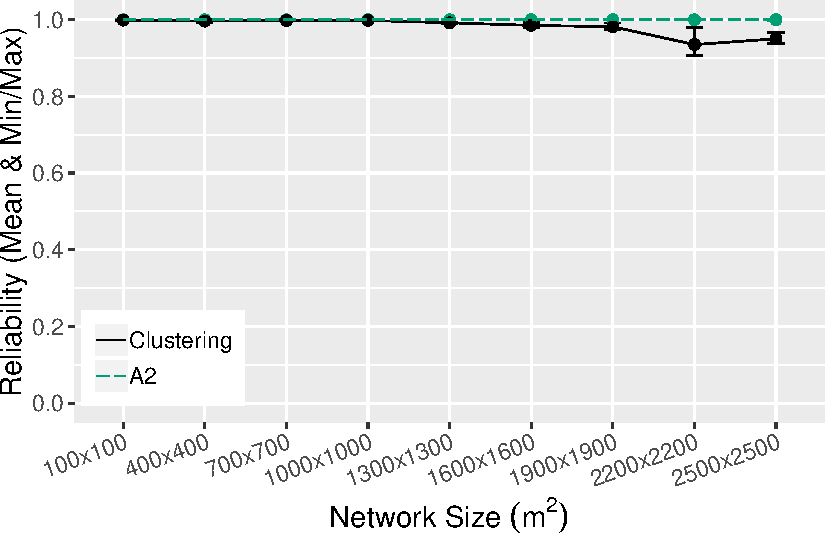
\includegraphics[width=0.45\textwidth]{figure/Results/ChaosComparison/ChaosComparison_50_Reliability.pdf}
            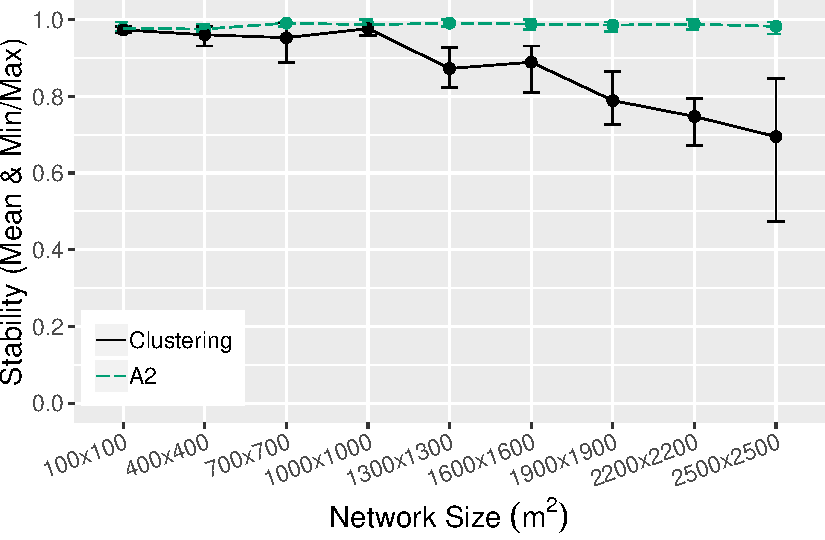
\includegraphics[width=0.45\textwidth]{figure/Results/ChaosComparison/ChaosComparison_50_Stability.pdf}
            \caption{Networks with 50 nodes.}
            \label{subfig:reliability-50-nodes}
    \end{subfigure}
    \hfill
    \begin{subfigure}{\textwidth}
        \centering
        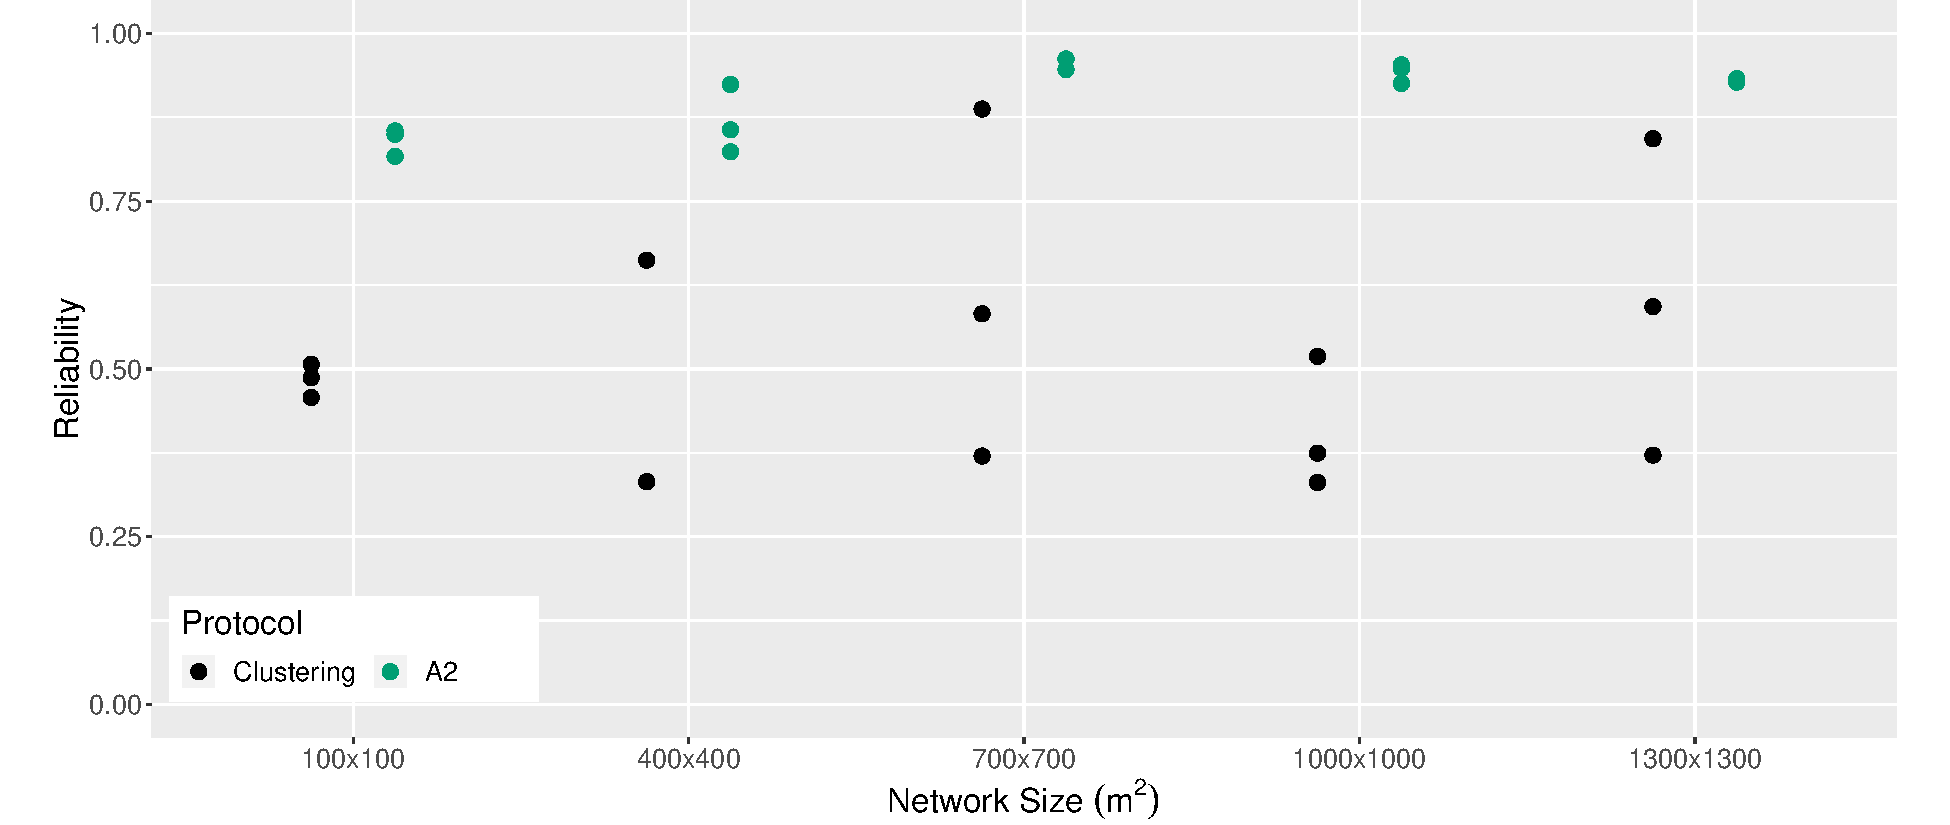
\includegraphics[width=0.45\textwidth]{figure/Results/ChaosComparison/ChaosComparison_200_Reliability.pdf}
        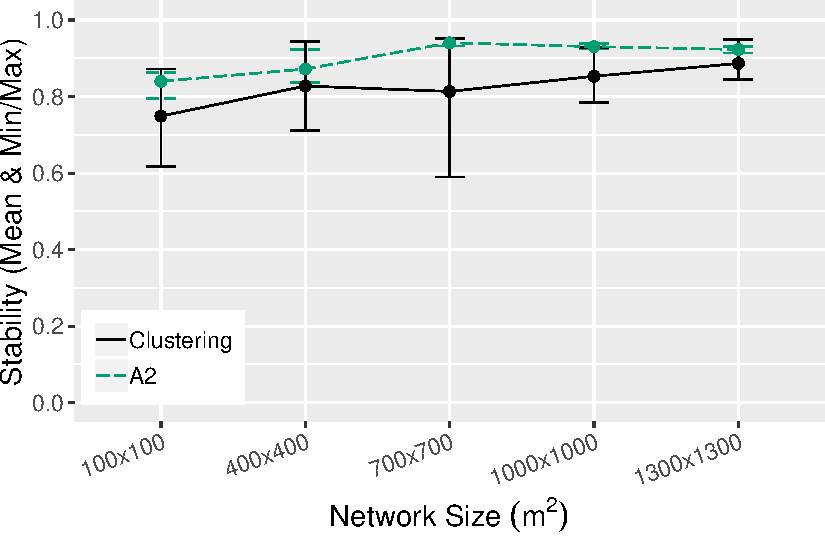
\includegraphics[width=0.45\textwidth]{figure/Results/ChaosComparison/ChaosComparison_200_Stability.pdf}
        \caption{Networks with 200 nodes.}
        \label{subfig:reliabilty-200-nodes}
    \end{subfigure}
    \caption{Reliability and stability comparison between \atwo{} with clustering and original \atwo{}.}
    \label{fig:reliability-result}
\end{figure}



\begin{figure}[bt]
    \centering
    \begin{subfigure}{0.45\textwidth}
        \centering
        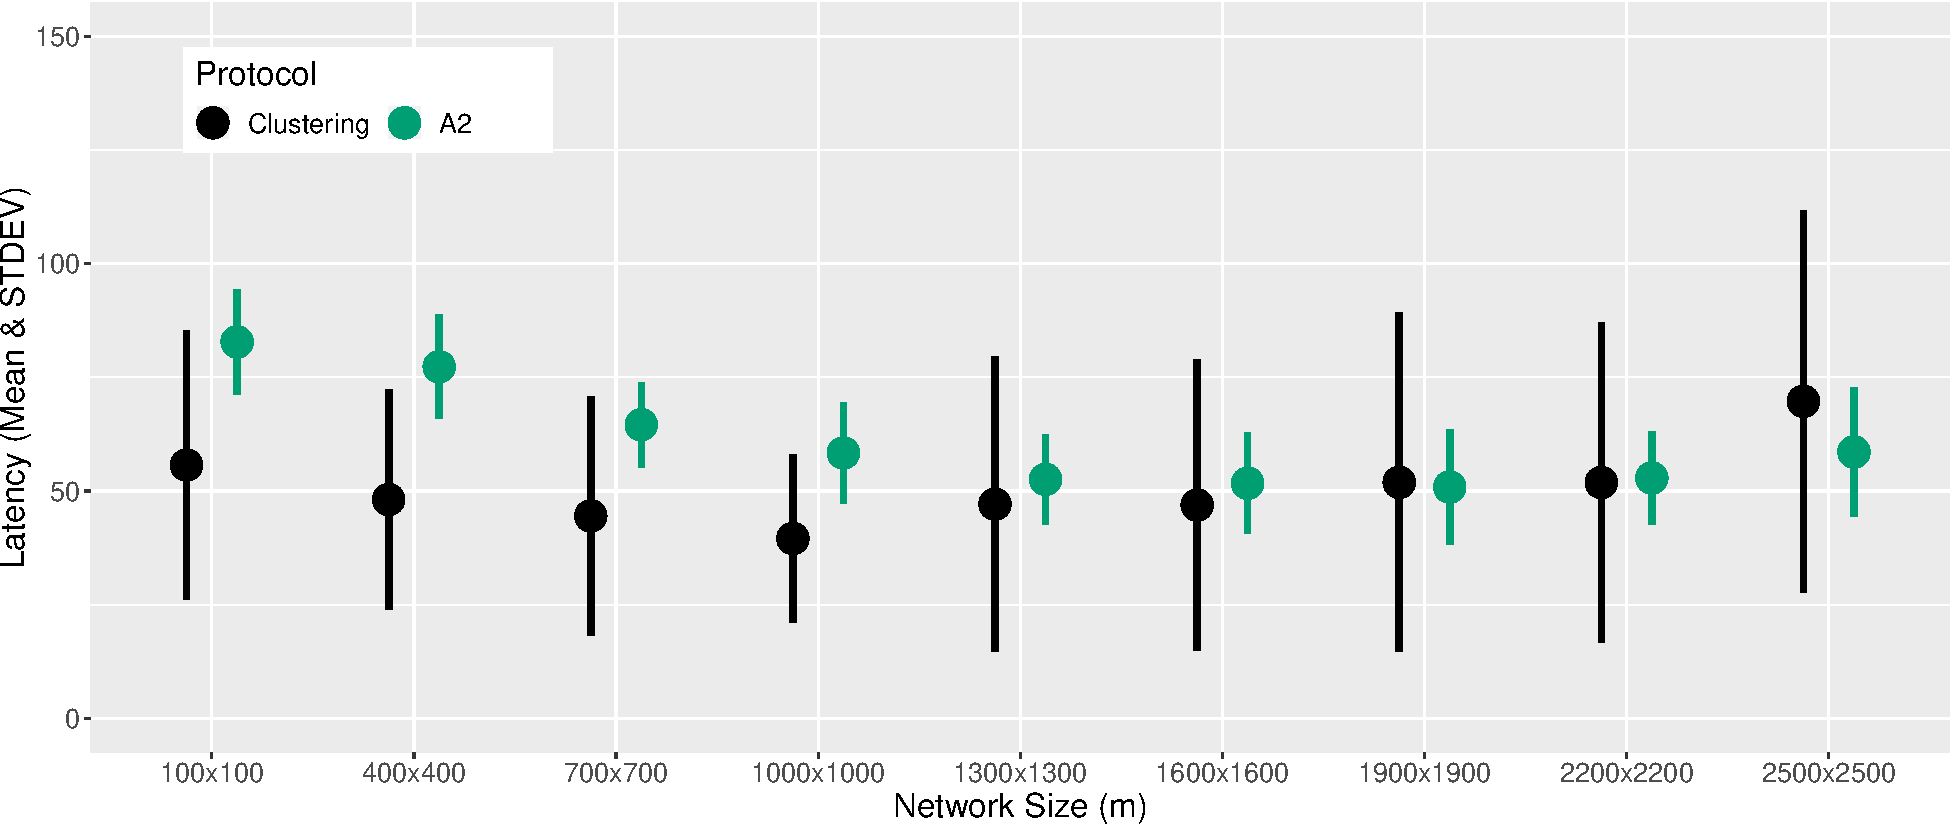
\includegraphics[width=\textwidth]{figure/Results/ChaosComparison/ChaosComparison_50_Latency.pdf}
        \caption{Networks with 50 nodes.}
        \label{subfig:latency-50-nodes}
    \end{subfigure}
    %\hfill
    \begin{subfigure}{0.45\textwidth}
        \centering
        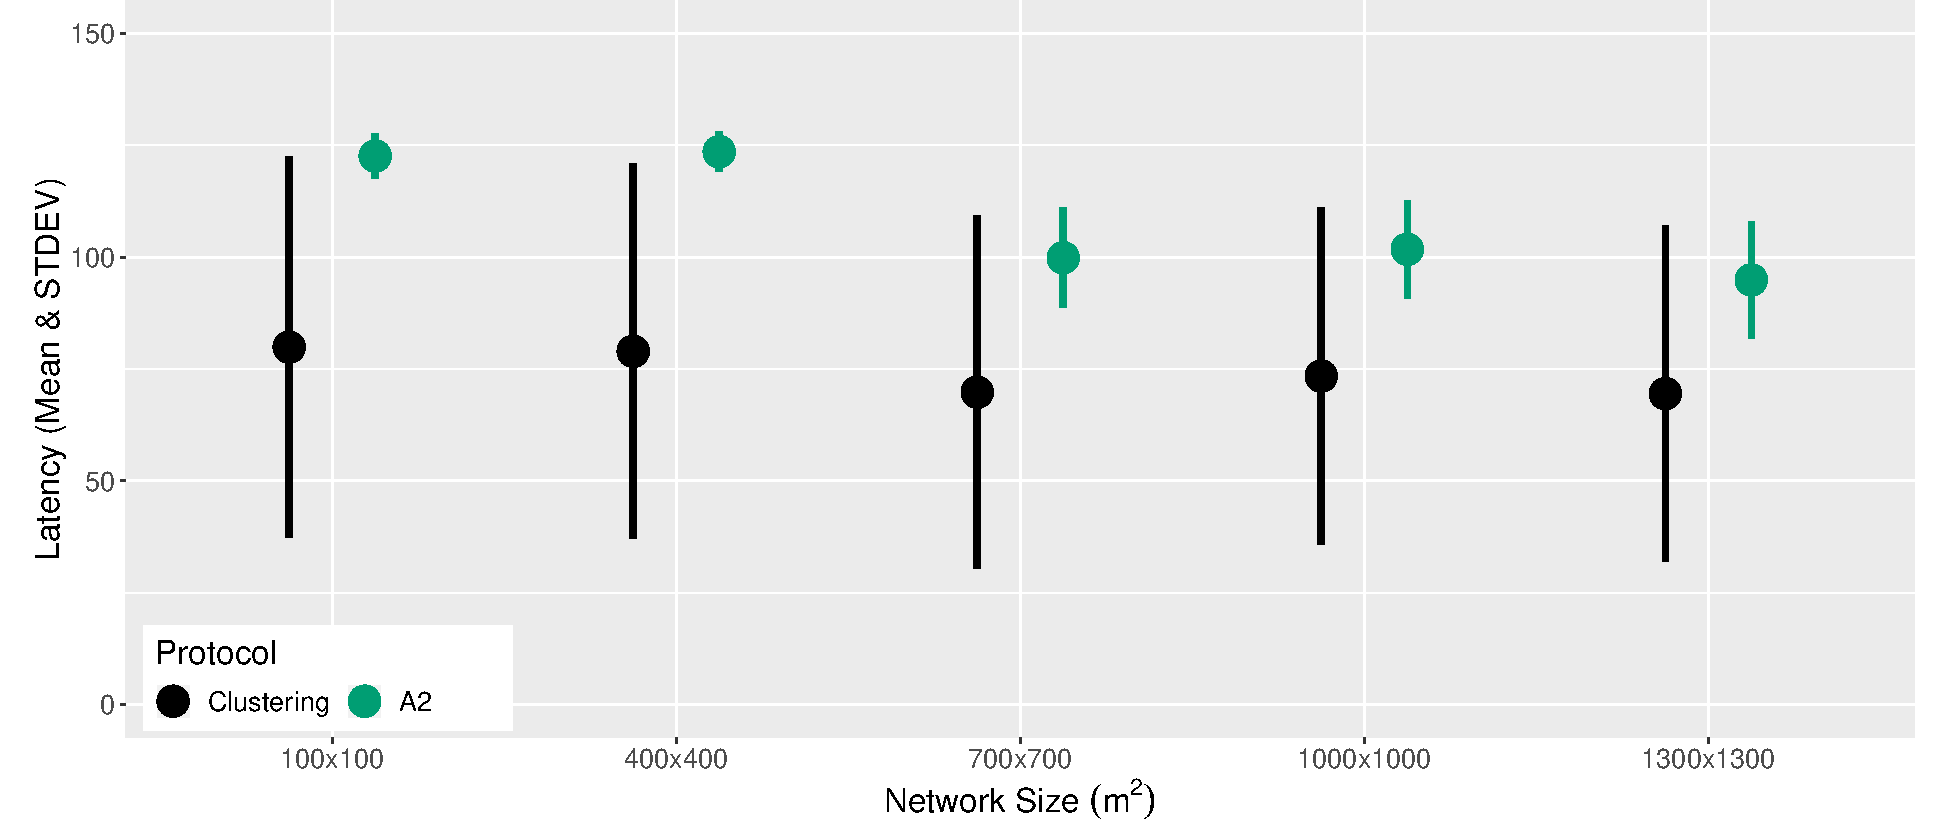
\includegraphics[width=\textwidth]{figure/Results/ChaosComparison/ChaosComparison_200_Latency.pdf}
        \caption{Networks with 200 nodes.}
        \label{subfig:latency-200-nodes}
    \end{subfigure}
    \caption{Latency comparison between \atwo{} with clustering and original \atwo{}.}
    \label{fig:latency-results}
\end{figure}


\subsection{Latency}
We show the mean latency and standard deviation for each test we run in \cref{fig:latency-results}. Looking at the tests using 50 nodes (\cref{subfig:latency-50-nodes}) the latency for the clustering implementation is on average a little lower for network topologies smaller than $2200x2200m^2$, after that the \atwo{} system outperforms our implementation. However, for all network topologies our clustering implementation has a higher standard deviation. We see a similar trend for 200 nodes (\cref{subfig:latency-200-nodes}), the standard deviation is still high; however, our clustering implementation consistently has a lower mean latency for all topologies tested. 

If we compare the latency between 50 nodes and 200 nodes, we see that it increases as the number of nodes increases. Consequently, we get lower latency when applying clustering since each cluster only contains a proportion of all nodes in the network.



\begin{figure}[bt]
    \centering
    \begin{subfigure}{0.45\textwidth}
        \centering
        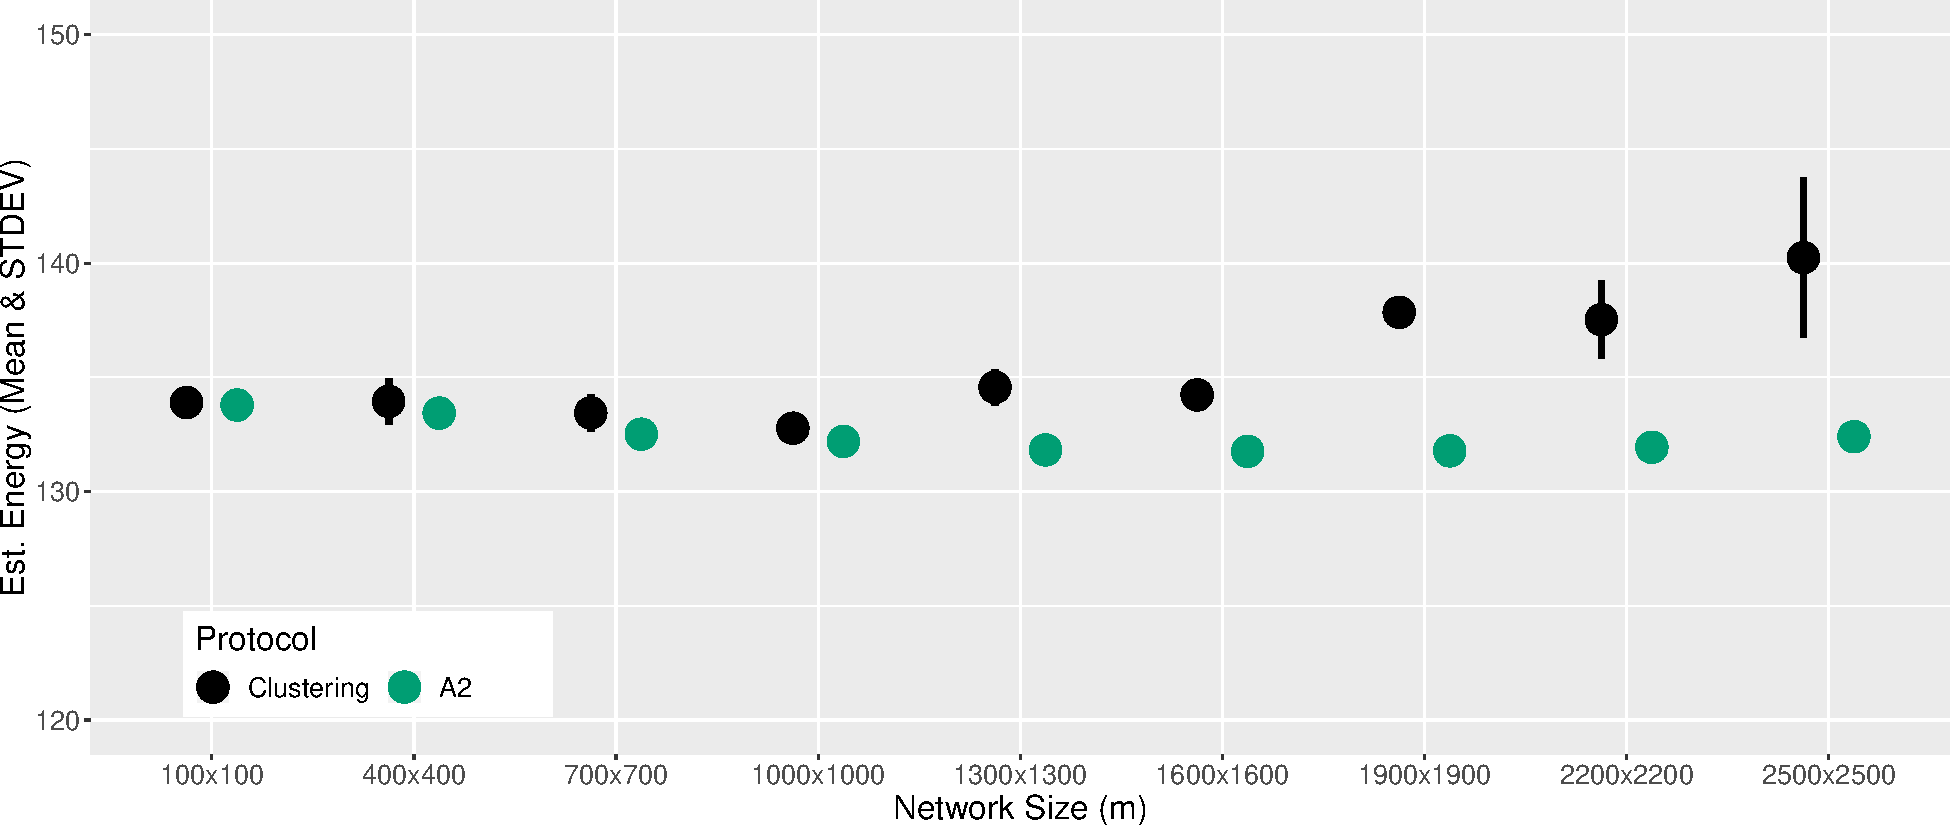
\includegraphics[width=\textwidth]{figure/Results/ChaosComparison/ChaosComparison_50_Energy.pdf}
        \caption{Networks with 50 nodes.}
        \label{subfig:energy-50-nodes}
    \end{subfigure}
    \begin{subfigure}{0.45\textwidth}
        \centering
        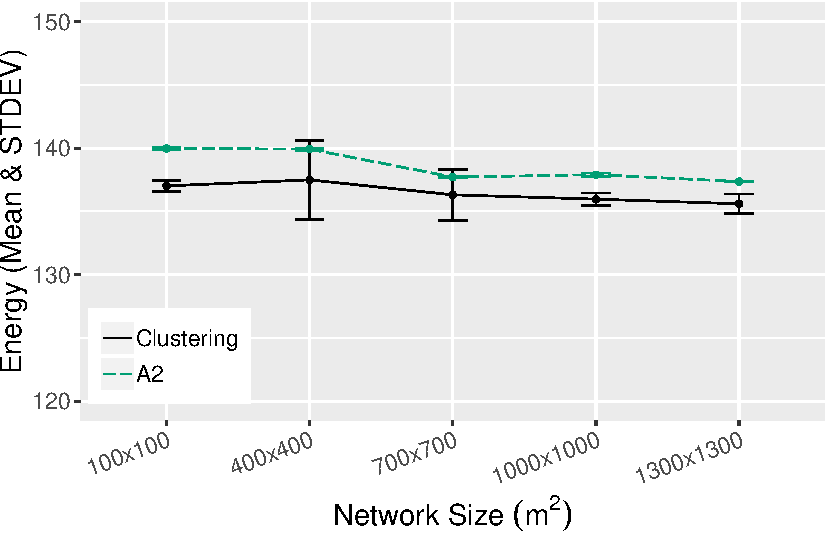
\includegraphics[width=\textwidth]{figure/Results/ChaosComparison/ChaosComparison_200_Energy.pdf}
        \caption{Networks with 200 nodes.}
        \label{subfig:energy-200-nodes}
    \end{subfigure}
    \caption{Energy comparison between \atwo{} with clustering and original \atwo{}.}
    \label{fig:energy-results}
\end{figure}


\subsection{Energy}
In \cref{fig:energy-results}, we show the mean energy usage per node per Energest time unit. We observe in \cref{subfig:energy-50-nodes} that energy usage for clustering increases with network area. We also observe that stability (\cref{subfig:reliabilty-200-nodes}) has an inverse relationship to energy usage, because an unstable node consumes more energy than a stable node. Both associating with the network and running the Join service requires more energy than the max application. They take more energy since the Join service takes longer time than the max application, and when a node associates it does not sleep.

Comparing 50 to 200 nodes we notice a higher energy usage on average for 200 nodes, which we expect to see since more nodes require more communication and longer rounds, which leads to higher energy consumption. Clustering shows a small advantage with 200 nodes \cref{subfig:energy-200-nodes}, compared to \atwo{}; each cluster can reach consensus in fewer slots than the whole network can, which is why the average energy usage is lower on all topologies.

Finally, the energy usage differs from the other metrics in that it is measured during both the coordination and application phase.  It is measured in all rounds because the energy results for only the applications could be misleading since the energy usage by the clustering process could outweigh the benefit of clustering the network.

\begin{figure}[bt]
    \centering
    \begin{subfigure}{0.24\textwidth}
        \centering
        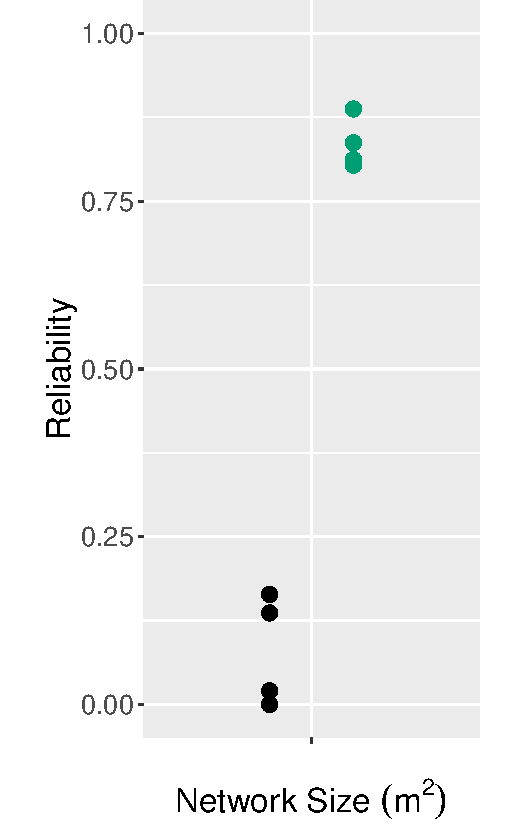
\includegraphics[width=\textwidth, keepaspectratio]{figure/Results/ChaosComparison/Flocklab/FlocklabComparison_Reliability.pdf}
        \caption{Reliability.}
        \label{subfig:flocklab-reliability}
    \end{subfigure}
    \begin{subfigure}{0.24\textwidth}
        \centering
        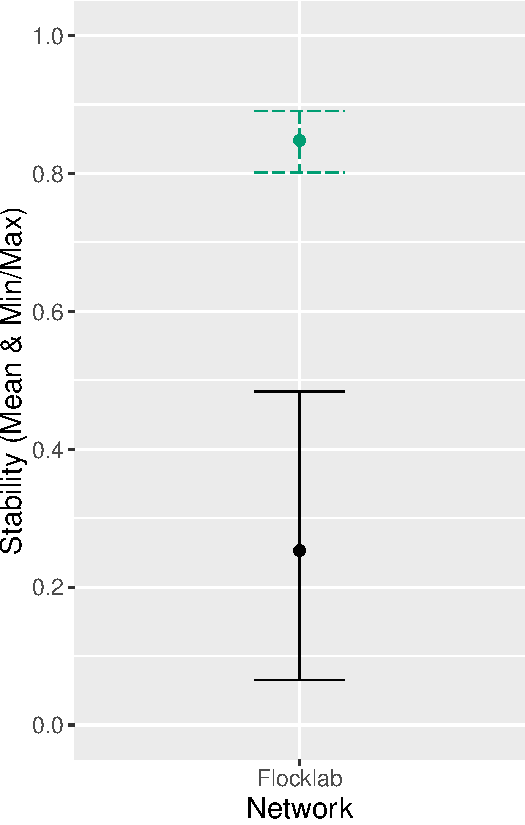
\includegraphics[width=\textwidth, keepaspectratio]{figure/Results/ChaosComparison/Flocklab/FlocklabComparison_Stability.pdf}
        \caption{Stability.}
        \label{subfig:flocklab-stability}
    \end{subfigure}
    \begin{subfigure}{0.24\textwidth}
        \centering
        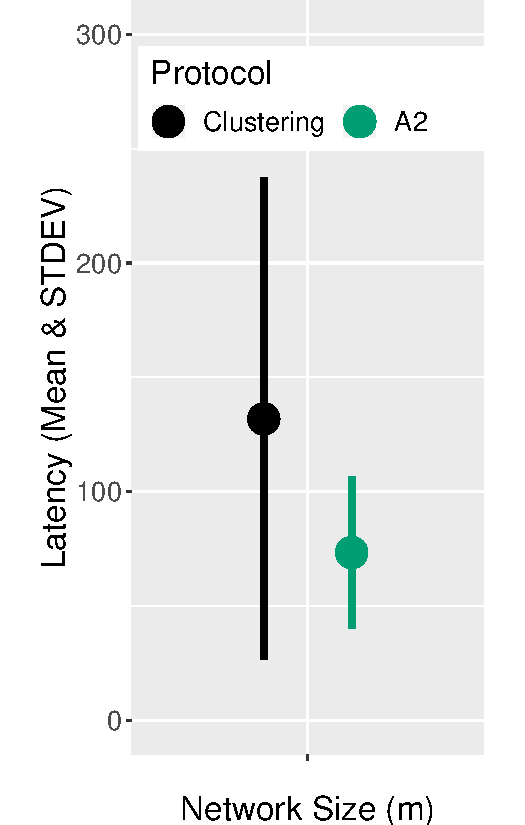
\includegraphics[width=\textwidth, keepaspectratio]{figure/Results/ChaosComparison/Flocklab/FlocklabComparison_Latency.pdf}
        \caption{Latency.}
        \label{subfig:flocklab-latency}
    \end{subfigure}
    \begin{subfigure}{0.24\textwidth}
        \centering
        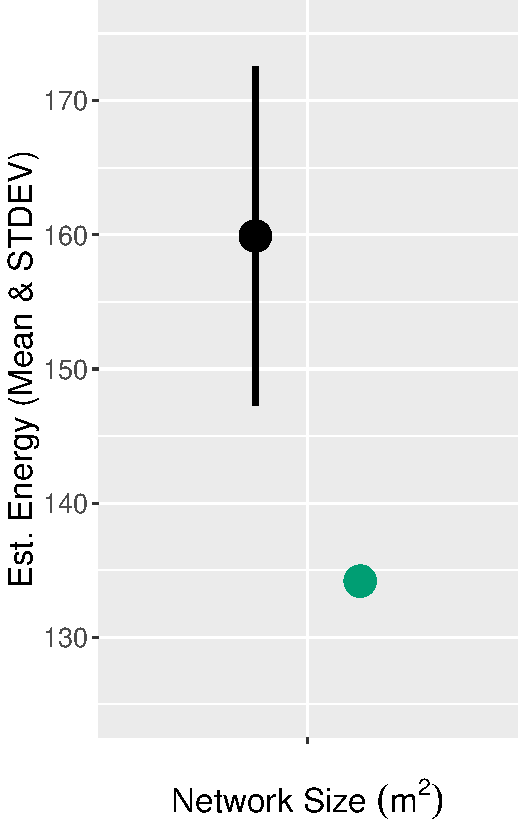
\includegraphics[width=\textwidth, keepaspectratio]{figure/Results/ChaosComparison/Flocklab/FlocklabComparison_Energy.pdf}
        \caption{Energy.}
        \label{subfig:flocklab-energy}
    \end{subfigure}
    \caption{The results of running \atwo{} and our clustering implementation on the Flocklab testbed. We show the mean and min/max for stability and reliability, and the mean and standard deviation for latency and energy consumption.}
    \label{fig:flocklab-results}
\end{figure}



\subsection{Flocklab}
We present the results from our tests on the Flocklab testbed in \cref{fig:flocklab-results}, which we get by running our clustering implementation and the \atwo{} system four times each. We see that \atwo{} outperforms our implementation in all metrics, achieving higher reliability and stability, lower latency, and lower energy consumption.

\begin{newtext}
Flocklab is a small and relatively sparse network with only 27 nodes, and it is also affected by external interference, which the simulations do not model. All of these factors contribute to lower stability, for both \atwo{} and the clustering implementation. 

When clustering the Flocklab network what often happens is that some node loses connection and need to associate with the network, to handle this the Join service is scheduled. Because no test run created more than two CHs, approximately half of the nodes begins to run the Join service, this makes it even harder for the other nodes to communicate, forcing more nodes to associate, creating a compounding effect of more and more nodes associating with the network. Nonetheless, running the clustering implementation on the Flocklab testbed demonstrates that the clustering process works when running on real nodes.
\end{newtext}


\section{Discussion}
\label{section:evaluation-discussion}
In this section, we discuss insights from our results. Furthermore, we discuss how our limitation on fault tolerance affected the stability of the networks. We also discuss running other applications in a clustered network, and end with some comments regarding the scalability and energy efficiency of a clustered network.


\subsection{Stability and Fault Tolerance}
\label{subsec:discussion-stability-and-fault-tolerance}
\begin{newtext}
From the results we get from comparing \atwo{} to our implementation, we see that our clustering implementation achieves similar reliability in almost all cases. However, the stability has high variance and is, in some cases, much lower. The primary reason for these stability results is that we did not consider fault tolerance for our clustering implementation. In this section, we will describe and discuss what scenarios lead to lower stability and how they relate to fault tolerance.



One of the most common fault tolerance issues is that a node loses connection to the network and has to re-associate with it. For a node, this process should look as follows.
    
\begin{enumerate}
    \item A node does not receive any packet for some rounds equal to \emph{round re-synchronisation threshold}.
    \item The node switches to association, listening for a packet with which it can synchronise.
    \item The node sets the join flag in outgoing packet headers, requesting that the initiator schedule the Join service.
    \item The current initiator schedules the Join service for its cluster.
\end{enumerate}

By analysing the tests from the comparison of our implementation to the \atwo{} system, we see that stability issues always occur in step 4 of this process. We performed this analysis by looking at the outcomes of tests in the simulator; we do not attach any details of this here since it is too extensive.

Properly scheduling the Join service is complicated since we change both which node is the initiator and which nodes communicate while switching between cluster and cluster head rounds. The most common scenario, exemplified in \cref{fig:scenario-one-bug-example}, is that a node, in this case node 17, sets its join flag during a CH round, this happens first in round 270 in the example, and forces the first CH to schedule the Join service. The problem is that it does not matter which cluster node 17 has joined, it is always the first cluster that schedules the Join service. Consequently, since node 17 never gets the chance to join, because the wrong cluster is running the Join service, this scenario continues until a reclustering is scheduled.

\end{newtext}
\begin{figure}[bt]
    \centering
    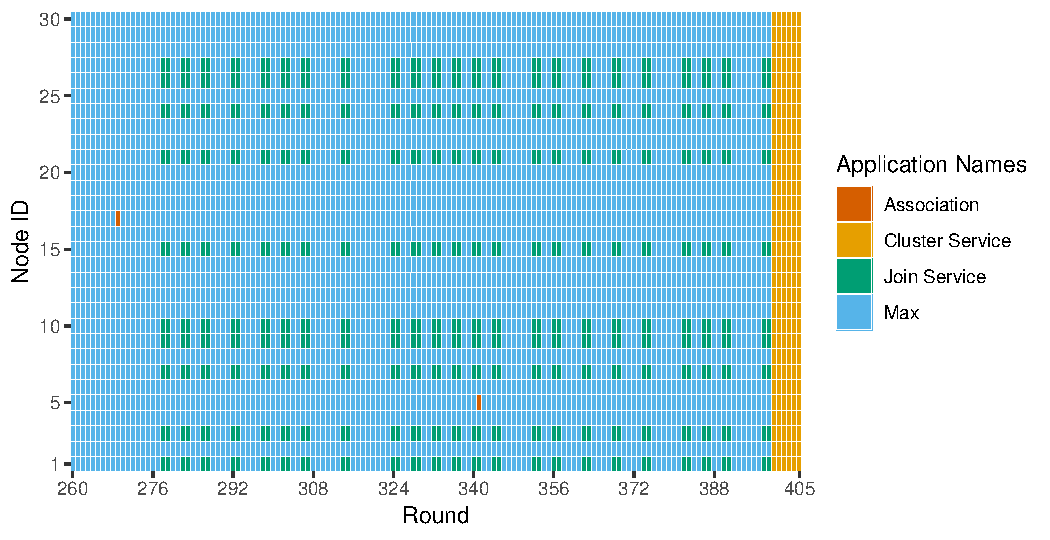
\includegraphics[width=0.75\textwidth] {figure/Results/Discussion/50NodesRun21000x1000Scenario1Example.pdf}
    \caption{Example of what happens when a node requests the Join service to be scheduled, blue is the correct application, green is the Join service, and yellow is the Clustering service. The first cluster repeatedly schedules the Join service without any effect.}
    \label{fig:scenario-one-bug-example}
\end{figure}


\begin{newtext}
Furthermore, if a CH loses connection to the network and has to associate, additional problems can occur. What happens depends on which CH associates. First, if the CH with the lowest ID associates, the network cannot continue normal execution, since that CH is the initiator during CH rounds. Causes and solutions to this problem are discussed more thoroughly in \cref{subsec:implementation_discussion-the-initiator}. Second, if another CH associates, the network will continue to execute the application. However, that node neither contributes its value nor sets its flag during CH rounds, which means the other nodes will never know that they have reached completion and cannot shut down early during CH rounds. This scenario does not impact the stability of the application, but it increases the latency and energy usage.

Finally, that our clustering implementation works in the absence of faults is supported by the reliability and stability results in \cref{fig:reliability-result}. Since the reliability metric does not include scenarios which require fault tolerance, it expresses the fact that clustering achieves good results during normal operation of the network. Additionally, from the stability results for 200 nodes, \cref{subfig:reliabilty-200-nodes}, we see that there are some tests which achieve better stability than \atwo{}, demonstrating that our clustering implementation has the potential to achieve better stability than the \atwo{} system in larger networks.
\end{newtext}


\subsection{Clustering Parameters}
\label{discussion:clustering-parameters}
The results we see in the parameter evaluation varies greatly, both when looking at a single test but also when looking at the different evaluations of the parameters combined. From the parameter evaluation, we can give some general remarks about each of the parameters.

\begin{newtext}
%Resync threshold discussion.
As we see in the resynchronisation threshold evaluation (\cref{subsec-resync-threshold}), both the stability and reliability increase significantly as the re-sync threshold increases. These results suggest that we should increase the re-sync threshold indefinitely. We did not evaluate this parameter further due to time constraints.


However, there are other reasons why indefinitely increasing this parameter will not yield the desired results. Re-sync threshold controls the number of rounds a node will wait while receiving no packets until it re-synchronises with the network again. Thus this parameter only fixes the symptom and not the cause of the problem, which is that a node has a bad connection to its cluster. For example, with a high re-sync threshold a node might stay in a suboptimal cluster since it receives enough packets to reset the re-sync threshold but not enough packets to complete the application running in the cluster, which will affect reliability.
\end{newtext}


For competition radius, we see that it is a parameter useful for creating reliable clusters since it had the most significant impact on the stability of a test for larger network areas.

For minimum cluster size, the results we got suggest that this parameter has a small impact on the overall stability. However, we see no correlation between the overall number of CHs and the stability, suggesting that these results either have some other underlying cause or the difference is due to noise. However, this parameter should be used, since it prevents clusters with only one node to form.

Last, the nodes per cluster ratio parameter worked as we expected. With a lower value of this parameter, we saw that the clustering process created more CHs. However, this parameter requires careful consideration since it can cause too many CHs to be created for sparse networks, as we see in \cref{subsec:nodes-per-cluster-ratio}.

\subsection{Running Other Applications in a Clustered Network}
\label{subsec:discuss-other-apps}
\begin{newtext}
Throughout this thesis, we limit our evaluation to the Max application. This limitation is because our focus was to implement clustering on top of the \atwo{} system, and not to see how different applications perform in a clustered network. However, we discuss how other applications may benefit from a hierarchical network to show that clustering is not limited to the Max application. Some common applications for a WSN include calculating a sum, mean, median, or performing a 2 or 3 phase commit. However, running applications in a clustered network require some adaptations, compared to a normal network.

Calculating a sum in a clustered network requires few adaptations from an implementation for a non-clustered network, however, it can take advantage of the hierarchical communication. Each CH would be able to calculate its cluster's sum of proposed values. CHs then repeat the same process during the CH round where they share their intermediary sum with all other CHs. However, one difference when calculating a sum compared to a maximal value is that a CH needs to maintain a list of all contributed values and which node contributed with what value. If the nodes were to add values together, then the same value could be added to the sum multiple times. Since \atwo{} has a restriction on the packet size, the number of nodes that can propose values is restricted. Clustering the network would directly help with this since smaller parts of the network calculate separate sums, which means the list of proposed values is smaller.

Furthermore, calculating the median in a clustered network require more resources than calculating a sum, since all values have to be known to at least one node. Clustering affects the size of the required list in each cluster in the same way as when calculating the sum. However, the CH cannot perform an intermediary calculation as in the sum application. The CHs will instead share the lists between each other, merging all lists from all clusters, which would result in a list with a length equal to the number of nodes in the network. Therefore, calculating the median in a clustered network compared to a non-clustered network does not scale better with regards to packet size.

However, calculating the mean can make efficient use of a clustered network. A mean calculation requires two things: the sum of all proposed values, and the number of proposed values. Because a CH already knows the size of its cluster, they can perform a mean calculation in the same way as the sum calculation, with the extension that the CHs calculate the sum of the cluster sizes. At the end of the CH round, all CHs know the sum of all proposed values and the sum of all cluster sizes and can, therefore, calculate the mean.

Two other applications, which are more complicated than mean, sum and median, are two and three phase commit. Adapting these to run on a clustered network is not as straightforward. These applications can take advantage of clustering in all phases, running some of the collection and dissemination in parallel in every cluster. However, coordination is required between the CHs when switching between phases. The complexity lies in switching which node is the initiator when switching between inter- and intra-cluster communication. Especially if we were to implement a solution which executes the whole commit protocol in one round. We discuss the problems with switching between initiators in a round in \cref{subsec:implementation_discussion-the-initiator}.

In conclusion, clustering should increase the performance and scalability for many applications running on a WSN. Even applications which require a global view of the network can benefit from hierarchical communication. However, further work is required to implement these applications to evaluate the effectiveness of the clustering implementation.

\end{newtext}

\subsection{Achieving Better Scalability}
\begin{newtext}
One of the primary goals of this thesis is to increase the scalability of the \atwo{} system. We do not have a metric for measuring scalability directly, however, using the combined information from all metrics we argue that we achieved our goal. From the latency and energy usage results, we saw that our solution achieved a lower latency and energy usage for networks with 200 nodes. Additionally, since we cluster the network before running the Join service, the restriction caused by the flags field is not applied until after the clusters are created. Thus,  we increase the theoretical maximum number of nodes in the network, and the restriction is now local to every cluster.

However, there are some caveats to achieving better scalability. First, we measure the latency results per round. We do not take into account that a clustered network requires two complete rounds to agree on a global maximum value, while \atwo{} only requires one round. A clustered network requires two rounds because we schedule the inter- and intra-cluster communication in separate rounds. Second, even though our implementation has lower stability than \atwo{} in almost all cases, we achieve better latency and lower energy usage; this is good since we achieve those results even in the presence of more faults.

Furthermore, low stability could imply less scalability as well. Our results suggest that the stability decreases as the number of nodes increase, however, we have shown that this is caused by our limitation on fault tolerance and is not inherent to clustering the network.

Despite these caveats, we argue that the results are promising. From the discussion on fault tolerance we conclude that we could attribute the drops in stability to our limitation on fault tolerance. If future work research and implement fault tolerance, our clustering implementation has a high probability of achieving equal or better stability while running more scalable and energy efficient networks.
\end{newtext}
